\chapter{Related Works}

Your related works, and your purpose and contribution which must be different as below.

\section{Fadila/1164072}
\subsection{Teori}
Penyelesaian Tugas Harian 3 ( No. 1-7 )
\begin{enumerate}
\item Binary Classification Dan Ilustrasi Gambarnya
\begin{itemize}
\item Pengertian Binary Classification / Klasifikasi Biner:
\par Klasifikasi biner atau binomial merupakan tugas untuk mengklasifikasikan elemen-elemen dari himpunan tertentu ke dalam dua kelompok (memprediksi kelompok mana yang masing-masing dimiliki) ber-
\par dasarkan aturan klasifikasi.
\item Ilustrasi Gambar Binary Classification :
\par

\begin{figure}[ht]
\centering
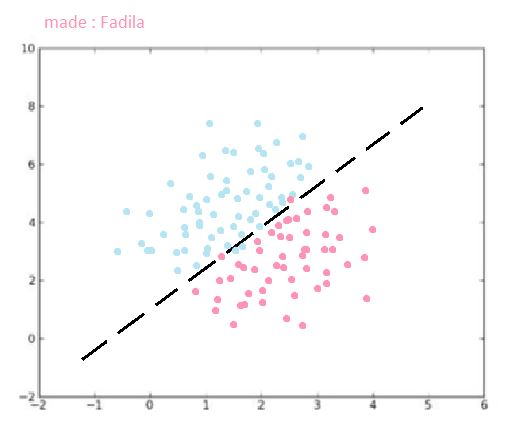
\includegraphics[scale=0.3]{figures/binary.jpg}
\caption{binary classification}
\label{contoh}
\end{figure}

\par
\end{itemize}
\item Supervised Learning, Unsupervised Learning, Clustering Dan Ilustrasi Gambar
\begin{itemize}
\item Pengertian Supervised Learning :
\par Sebuah pendekatan dimana terdapat data yang dilatih dan ditargetkan. Leih singkatnya supervised learning memiliki kategori sehingga tujuan dan outputnya jelas.
\begin{itemize}
\par
\item Ilustrasi Gambar Supervised Learning :

\begin{figure}[ht]
\centering
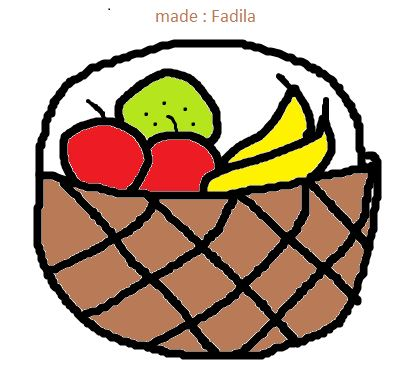
\includegraphics[scale=0.4]{figures/supervised1.jpg}
\caption{supervised}
\label{contoh}
\end{figure}


\par Pada contoh gambar diatas dikelompokkan bahwa apabila bentuk dari objek di gambar berbentuk bundar dan berwarna merah maka akan dinamakan atau di sebut sebagai Apel. Dan apabila pada gambar terdapat objek berbentuk panjang dan berwarna kuning maka akan dinamakan atau di sebut sebagai pisang.
\par
\end{itemize}

\par
\item Pengertian Unsupervised Learning :
\par Tidak memiliki data latih, sehingga dari data yang tersebut kita bisa mengelompokkannya ke berbagai kelompok 2 seterusnya. Dengan lebih singkatnya ialah unsupervised learning tidak memiliki kategori.
\par
\par
\begin{itemize}
\item Ilustrasi Gambar Unsupervised Learning :

\begin{figure}[ht]
\centering
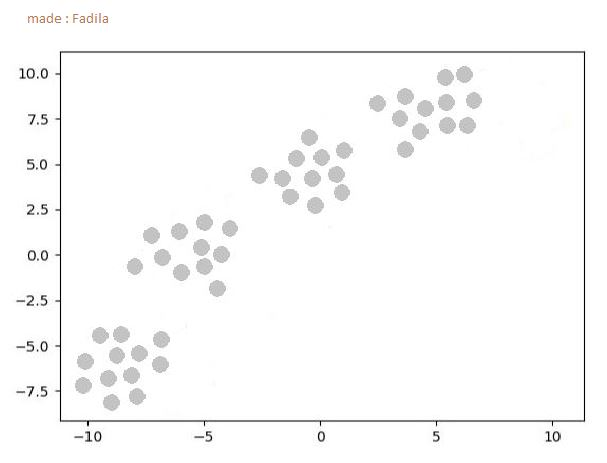
\includegraphics[scale=0.4]{figures/unsupervised2.jpg}
\caption{unsupervised}
\label{contoh}
\end{figure}

\par Pada gambar dapat dilihat bahwa ada banyak data namun tidak pada pengelompokkan yang tepat. Cuman dapat dikelompokkan ke dalam berbagai macam bentuk dan jumlah namun tidak memberikan output yang jelas.
\par
\par
\end{itemize}
\item Pengertian Clustering :
\par Metode pengelompokan data. Clustering juga merupakan proses partisi satu set objek data ke dalam himpunan bagian yang disebut dengan cluster. Objek dalam cluster tersebut memiliki kemiripan karakteristik antar satu sama lain.
\par

\begin{figure}[ht]
\centering
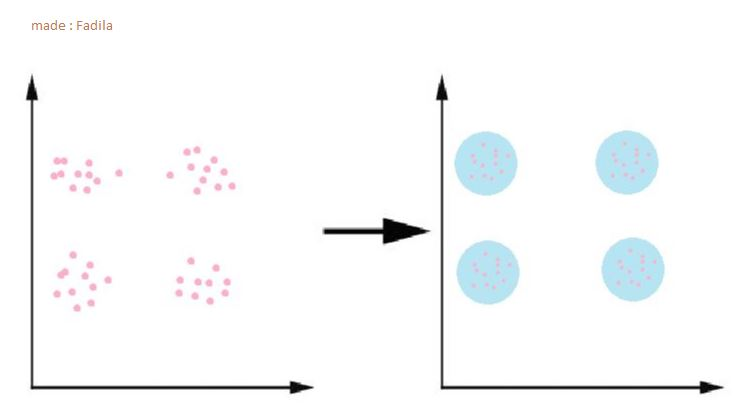
\includegraphics[scale=0.5]{figures/clustering.jpg}
\caption{clustering}
\label{contoh}
\end{figure}

\par
\end{itemize}
\item Evaluasi, Akurasi Dan Ilustrasi Gambar
\begin{itemize}
\item Pengertian Evaluasi
\par Evaluasi digunakan untuk memeriksa/memastikan dan mengevaluasi model dalam bekerja ( seberapa baik ) dengan mengukur keakuratannya. Kita juga dapat menanalisis kesalahan yang dibuat pada model yang dijalankan, tingkat kebingungan dan menggunakan matriks kebingunan.
\par

\begin{figure}[ht]
\centering
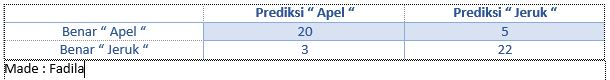
\includegraphics[scale=0.6]{figures/eva.jpg}
\caption{Evaluasi}
\label{contoh}
\end{figure}

\par Pada contoh gambar dapat dilihat bahwa dilakukan evaluasi terhadap kerja dalam penentuan jenis dari objek. Dievaluasi berapa banyak sebuah objek ketika dikelompokkan dan diklasifikasikan kemudian dapat dilihat apakah kerjanya sesuai atau tidak.
\par

\par
\item Pengertian Akurasi
\par Accuracy akan didefinisikan sebagai presentasi kasus yang diklasifikasikan dengan benar. Accuracy lebih jelasnya adalah perbandingan kasus yang diidentifikasi benar dengan jumlah semua kasus
 \par Rumus dari accuracy= (a+c)/(a+b+c+d)
\par

\begin{figure}[ht]
\centering
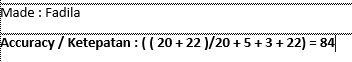
\includegraphics[scale=0.8]{figures/acuracy.jpg}
\caption{Akurasi}
\label{contoh}
\end{figure}

\par Dilakukan perhitungan dengan rumus akurasi terhadap data yang telah diolah pada " Evaluasi ". Kemudian di dapatkan hasil dari pengolahan data tersebut.
\par Contoh penggabungan Akurasi Dan Evaluasi
\par

\begin{figure}[ht]
\centering
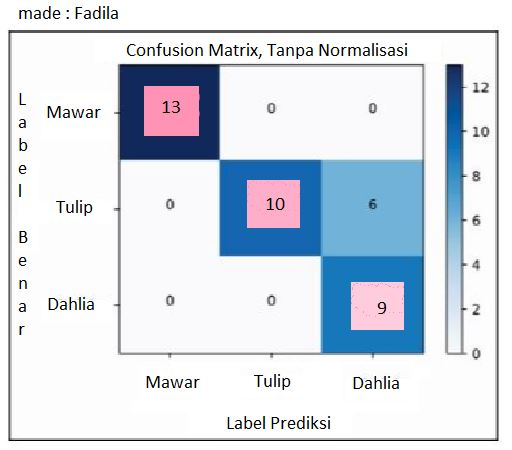
\includegraphics[scale=0.5]{figures/evacuray.jpg}
\caption{Contoh Evaluasi Dan Akurasi Secara Bersamaan }
\label{contoh}
\end{figure}

\end{itemize}

\par
\item Membuat Dan Membaca Confusion Matrix Beserta Contoh
\begin{itemize}
\item Pengertian Confusion Matrix
\par Confusion matrix merupakan suatu metode yang  digunakan untuk melakukan perhitungan akurasi pada konsep data mining.
\par
\item Pembacaan Confusion Matrix
\begin{enumerate}
\item Apabila hasil prediksi negatif dan data sebenarnya merupakan negatif.
\item Apabila hasil prediksi positif sedangkan nilai sebenarnya merupakan negatif.
\item Apabila hasil prediksi negatif sedangkan nilai sebenarnya merupakan positif.
\item Apabila hasil prediksi positif dan nilai sebenarnya merupakan positif.
\end{enumerate}
\par
\par
\item Pembuatan Confusion Matrix
\begin{enumerate}
\item Menentukan 4 proses klasifikasi yang akan digunakan dalam confusion matrix.
\item 4 Istilah tersebut ada True Positive ( TP ), True Negative ( TN ), False Positive ( FP ) dan False Negative ( FN ).
\item Kelompokkan klasifikasi tersebut bisa menggunakan klasifikasi biner
\item Akan menghasilkan keluaran berupa 2 Kelas ( Positif dan Negatif ) dan penentuan TP, FP ( 1 klasifikasi positif ) , FN dan TN ( 1 klasifikasi negatif ).
\item Contoh dasarnya nampak seperti langkah diatas
\item Istilahnya daat didefinisikan dengan objek lain namu dengan alur yang sama ( sesuai rumus baik klasifikasi dll ).
\end{enumerate}
\par

\item Ilustrasi Gambar
\par

\begin{figure}[ht]
\centering
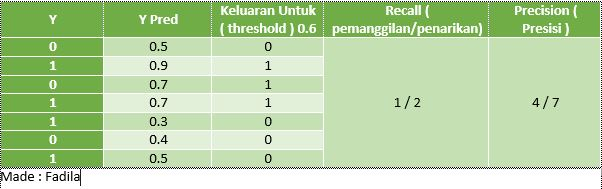
\includegraphics[scale=0.6]{figures/confusion.jpg}
\caption{confusion matrix}
\label{contoh}
\end{figure}

\par
\begin{itemize}
\item Penjelasan
\begin{enumerate}
\item Recall
\par Dari semua kelas positif, seberapa banyak yang kami prediksi dengan benar. Itu harus setinggi mungkin.
\par

\begin{figure}[ht]
\centering
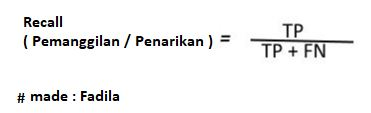
\includegraphics[scale=0.6]{figures/recall.jpg}
\caption{recall}
\label{contoh}
\end{figure}

\par
\item Presisi / Precision
\par Dari semua kelas, seberapa banyak yang kami prediksi dengan benar. Itu harus setinggi mungkin.
\par

\begin{figure}[ht]
\centering
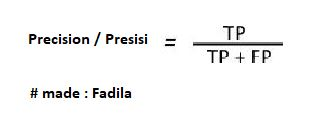
\includegraphics[scale=0.6]{figures/precision.jpg}
\caption{precision}
\label{contoh}
\end{figure}

\par
\item F-Ukur ( measure )
\par Sulit untuk membandingkan dua model dengan presisi rendah dan daya ingat tinggi atau sebaliknya. Jadi untuk membuatnya sebanding, kami menggunakan F-Score. F-score membantu mengukur Recall dan Precision pada saat yang bersamaan
\par

\begin{figure}[ht]
\centering
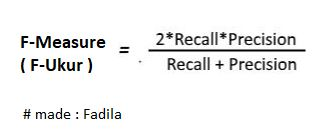
\includegraphics[scale=0.6]{figures/f.jpg}
\caption{f-measure}
\label{contoh}
\end{figure}

\par
\end{enumerate}
\end{itemize}
\end{itemize}


\par
\item Cara Kerja K-Fold Classification Dan Ilustrasi Gambar
\begin{enumerate}
\item Pertama-tama untuk total instance dibagi menjadi N bagian.
\item Fold ke-1 ( atau pertama ) adalah ketika bagian ke-1 menjadi data uji (testing data) dan sisanya menjadi data latih (training data).
\item Hitung akurasi ( berdasarkan porsi data tersebut. Persamaanya sebagai berikut :
\par (sigma) data klasifikasi
\par (sigma) total data uji
\par x 100 persen 
\item Fold ke-2 ( kedua ) adalah ketika bagian ke-2 menjadi data uji (testing data) dan sisanya menjadi data latih (training data). 
\item Kemudian dihitunglah akurasi berdasarkan porsi data yang telah ditentukan
\item Demikian seterusnya hingga mencapai fold ke-K. Hitung rata-rata akurasi dari K buah akurasi di atas. Rata-rata akurasi ini menjadi akurasi final atau akhir.
\end{enumerate}
\par
\begin{itemize}
\item Ilustrasi Gambar
\par

\begin{figure}[ht]
\centering
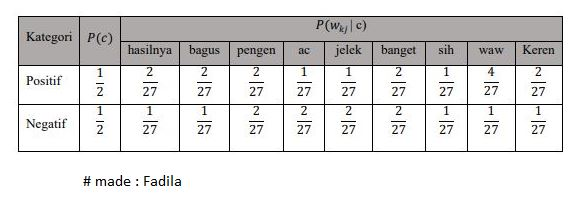
\includegraphics[scale=0.4]{figures/hasilk1.jpg}
\caption{k-fold classification 1}
\label{contoh}
\end{figure}

\begin{figure}[ht]
\centering
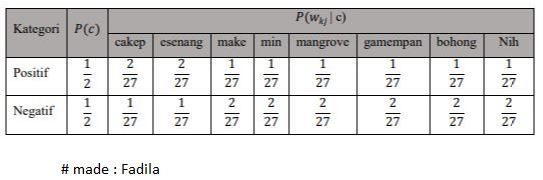
\includegraphics[scale=0.4]{figures/hasilk2.jpg}
\caption{k-fold classification 2}
\label{contoh}
\end{figure}

\par
\par
\end{itemize}

\par
\item Decision Tree Dan Ilustrasi Gambar
\begin{itemize}
\item Pengertian Decision Tree
\par Decision tree adalah salah satu metode klasifikasi yang paling populer karena mudah diinterpretasikan oleh manusia. Decision tree merupakan metode klasifikasi yang digunakan untuk pengenalan pola dan termasuk dalam pengenalan pola secara statistik. 3 tipe dari decision tree ialah:  simpul: simpul root, simpul perantara, dan simpul leaf.
\par

\end{itemize}
\par

\par
\begin{itemize}
\item Ilustrasi Gambar
\par


\begin{figure}[ht]
\centering
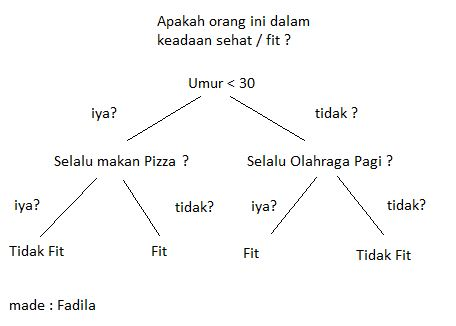
\includegraphics[scale=0.5]{figures/decisiontree.jpg}
\caption{decision tree}
\label{contoh}
\end{figure}

\par
\end{itemize}
\item Information Gain Dan Entropi
\begin{itemize}
\item Pengertian Information Gain
\par Information Gain adalah salah satu atribute selection measure yang digunakan untuk memilih test atribute tiap node pada tree.
\par Algoritme Information Gain digunakan untuk mengurangi dimensi atribut untuk mendapatkan atribut-atribut yang relevan. 
\par

\begin{itemize}
\item Ilustrasi Gambar
\par


\begin{figure}[ht]
\centering
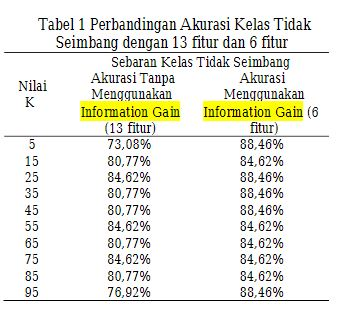
\includegraphics[scale=0.6]{figures/information1.jpg}
\caption{informaion gain 1}
\label{contoh}
\end{figure}


\begin{figure}[ht]
\centering
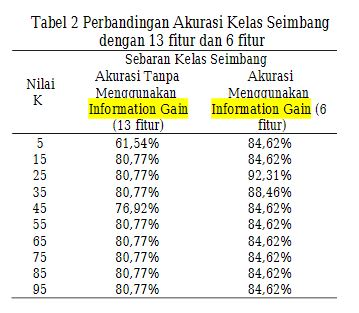
\includegraphics[scale=0.6]{figures/information2.jpg}
\caption{information gain 2}
\label{contoh}
\end{figure}

\item Penjelasan :
\par Tabel  1  sampai  dengan  Tabel  2 menunjukkan  bahwa  penggunaan  seleksi fitur Information  Gain  menghasilkan  nilai  akurasi yang  lebih  baik  dibandingkan  tanpa menggunakan Information Gain. 
\par Pada saat nilai K sama dengan 5 ( K=5) akurasi  yang  dihasilkan  sistem  tanpa menggunakan  Information  Gain  menunjukkan hasil  yang  kurang  baik  pada  sebaran  kelas seimbang maupun tak seimbang yaitu  61,54 persen pada sebaran kelas seimbang dan 73,08 persen pada sebaran  kelas tidak  seimbang. 
\end{itemize}


\par
\item Pengertian Entropi
\par Entropi pada umumnya merupakan salah satu besaran yang mengukur energi dalam sistem per satuan temperatur yang tak dapat digunakan untuk melakukan usaha.
\par Namun, secara spesifik untuk " Entropi " sendiri merupakan parameter untuk mengukur tingkat keberagaman (heterogenitas) dari kumpulan data. 

\par

\begin{figure}[ht]
\centering
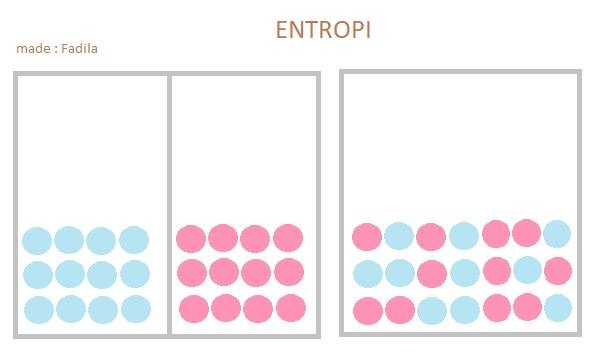
\includegraphics[scale=0.5]{figures/entropi.jpg}
\caption{entropi}
\label{contoh}
\end{figure}

\par
\end{itemize}

\end{enumerate}

\subsection{Topic 2}
if you have two topics you can include here to


\section{Same Method}
write and cite latest journal with same method

\subsection{Method 1}
cite and paraphrase method 1

\subsection{Method 2}
cite and paraphrase method 2 if you have more method please add new subsection.

 
>>>>>>> 31a49f1aef81f31f8ac75b18edbbc2dfd0fc6b2b
